\documentclass[a4paper,12pt]{report}

\usepackage{alltt, fancyvrb, url}
\usepackage{graphicx}
\usepackage[utf8]{inputenc}
\usepackage{float}
\usepackage{hyperref}

% Questo commentalo se vuoi scrivere in inglese.
\usepackage[italian]{babel}

\usepackage[italian]{cleveref}

\newcommand{\gametitle}{Ciccio Pier - THE GAME}

\title{Relazione per\\``\gametitle''}

\author{
    Alessandro Aldini
    \and
    Davide Valdifiori
    \and
    Riccardo Mingozzi
    \and
    MD Shokot Alam
}

%\date{Anno Accademico 2021/2022}
\date{25 aprile 2022}


\begin{document}

    \maketitle

    \tableofcontents

    \chapter{Analisi}

    Il software realizzato per il corso di Programmazione ad Oggetti è \gametitle, un videogioco ispirato a Super Mario Bros. L'obbiettivo del gioco è superare i livelli, con difficoltà progressiva, cercando di ottenere il punteggio più alto possibile.

    La difficoltà del gioco consiste nel superare vari ostacoli, tra cui nemici, trappole, platforming e gestire il sistema della stamina.

    \section{Requisiti}

    \subsubsection{Requisiti funzionali}
    \begin{itemize}
        \item Inserire il proprio username per salvare il punteggio ottenuto a fine livello e visualizzare la classifica con i punteggi migliori
        \item Vari livelli con ambientazioni differenti e difficoltà crescente
        \item Possibilità di cambiare le impostazioni di gioco ad esempio suoni, risoluzione, etc...
        \item Tutorial all'interno del gioco
        \item Diversi tipi di nemici con comportamenti ed attacchi differenti
        \item Il giocatore può attaccare i nemici con l'azione del morso
        \item Il giocatore perde vita quando viene attaccato dai nemici o mangiando cibi grassi, può recuperarla uccidendo i nemici
        \item Il giocatore perde stamina saltando, può recuperarla mangiando nemici o cibi grassi. Se la stamina scende sotto un certo livello il giocatore sarà svantaggiato nel movimento
        \item I boosts conferiscono vantaggi al giocatore
        \item Il punteggio ottenuto a fine livello è dato da quanti nemici sono stati uccisi e dal numero di oggetti raccolti, che sono boosts, cibi e monete
    \end{itemize}

    \subsubsection{Requisiti non funzionali}
    \begin{itemize}
        \item Il gioco dovrà avere una grafica intuitiva e accattivante
        \item Il gioco dovrà avere musiche ed effetti sonori per migliorare l'esperienza di gioco
    \end{itemize}

    \section{Analisi e modello del dominio}

    Il gioco è formato da vari livelli.

    Ogni livello è composto da un inizio che è il punto dove viene creato il giocatore, una fine che è il punto da raggiungere per poter completare il livello, dei nemici e degli oggetti da raccogliere .

    Il gioco dovrà essere in grado di accedere a tutti gli elementi del livello corrente ed essi dovranno poter interagire fra loro.

    Trattandosi di un platform, bisognerà sviluppare un adeguato ambiente di
    gioco, avente una corretta fisica, nemici con pattern di movimento prestabiliti
    e idonea iterazione tra gli elementi a schermo.

    Dovremo implementare concetti fisici di base come forza di gravità, fisicità
    degli oggetti e corretto funzionamento delle forze in campo, come ad esempio il salto.
    Un altro ostacolo potrebbe riguardare la gestione delle collisioni tra gli elementi.

    Avremo necessità dunque di controllare quello che accade nel gioco ripetitivamente senza pesare troppo sulle prestazioni. Il quantitativo di elementi a schermo potrebbe infatti risultare elevato, andrà trovato un modo efficace di gestire parallelamente tutti i nemici e il giocatore (mosso dall'utente tramite input).

    Il sistema di movimento dei nemici dovrà attivamente cercare il giocatore per attaccarlo e compiere movimenti che non li porti a uscire dal mondo o ad auto eliminarsi.

    \begin{figure}[H]
        \centering{}
        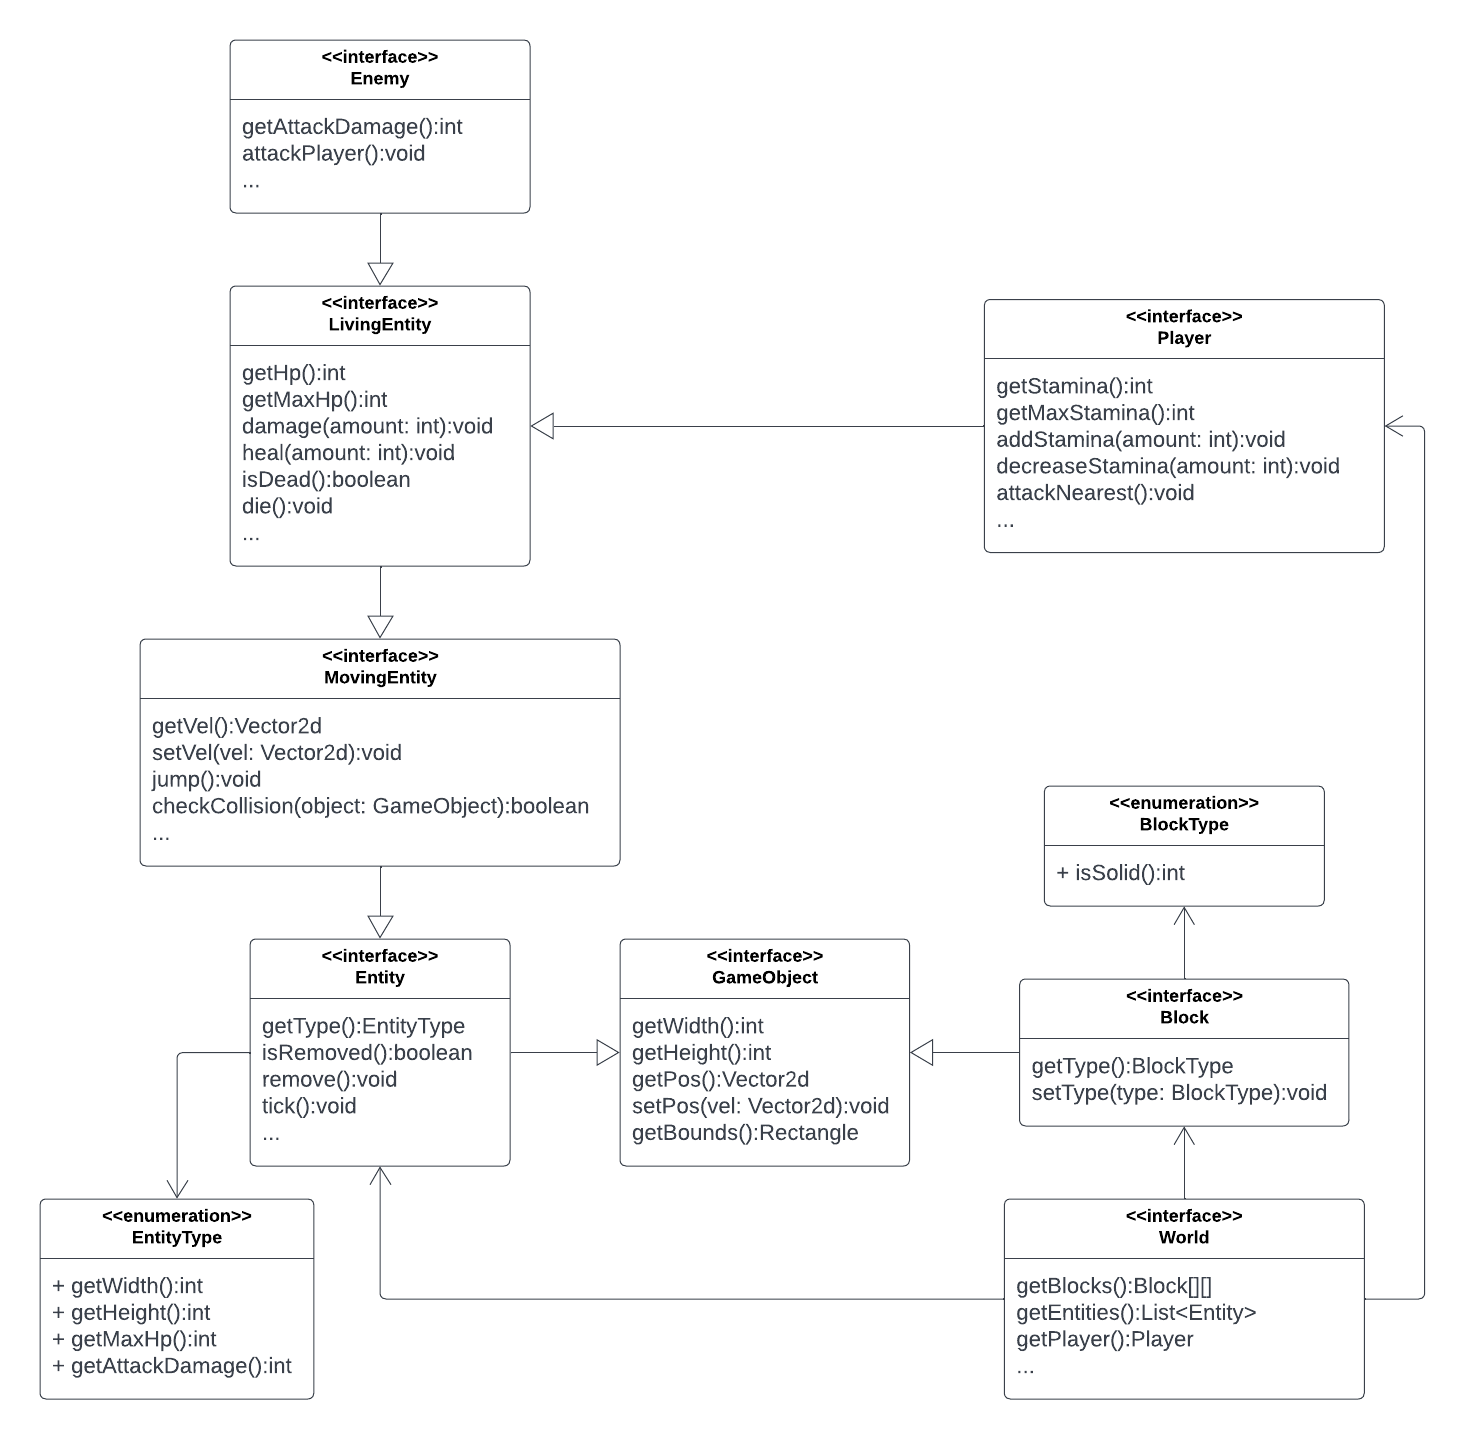
\includegraphics[scale=0.6] {img/analisi-uml.png}
        \caption{Schema UML delle entità del livello, con rappresentate le entità principali ed i rapporti fra loro}
        \label{img:analisi-uml}
    \end{figure}

    \chapter{Design}

    \section{Architettura}

    \begin{figure}[H]
        \centering{}
        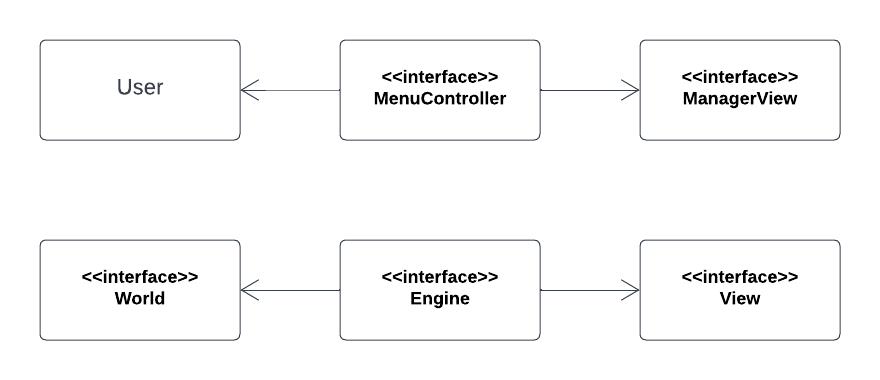
\includegraphics[scale=0.8] {img/architettura-uml.png}
        \caption{Rappresentazione UML dei patterns MVC utilizzati.}
        \label{img:users}
    \end{figure}

    Per realizzare l'applicazione è stato scelto di fare uso del pattern architetturale MVC.

    L'implementazione del menu di gioco sfrutta il pattern MVC ed è formato delle interface MenuController e ManagerView. Quando si avvia uno specifico livello, viene istanziato un sistema MVC dedicato.

    Tutti gli oggetti del livello vengono creati nel Model. Qui sono definite le caratteristiche e il comportamento degli oggetti principali: il Player, i blocchi e le entità. Nel pattern MVC la componente Model non conosce le altre due, per questo motivo al suo interno non vi sono riferimenti ad esse. Nel caso di "Ciccio Pier", il punto di ingresso al Model è rappresentato dall'implementazione dell'interfaccia World con la classe GameWorld.

    La componente Controller rappresenta il filo conduttore fra Model e View, ha il compito di manipolare le informazioni fornite dal Model e comunicarle alla View. Per gestire le iterazioni tra le componenti del gioco è stata implementata l'interfaccia classe Loop (GameLoop), che modella un vero e proprio game loop. Nel caso di "\gametitle", il controller è rappresentato dall'implementazione dell'interfaccia Engine con la classe GameEngine.

    La componente View ha il compito di rappresentare a schermo tutti gli oggetti del gioco rappresentando le componenti tramite immagini in Swing e di intercettare gli input dell'utente servendosi di un KeyListener per poi comunicarli al controller. Nel caso di "Ciccio Pier", la view è rappresentata dell'implementazione dell'interfaccia View con la classe GameView.

% ###IMMAGINE QUA!!

    \section{Design dettagliato}

    \subsection*{Alessandro Aldini}

    In questa sezione si analizzerà la struttura del menu principale e dei problemi che sono stati risolti durante la sua creazione, verranno inoltre citati aspetti come la gestione delle impostazioni di gioco e il funzionamento del ridimensionamento dello schermo in quanto facenti parte del contributo apportato al progetto.

    Il menu principale si basa sul pattern MVC, composto come segue:

    \subsubsection{Model}

    \begin{figure}[H]
        \centering{}
        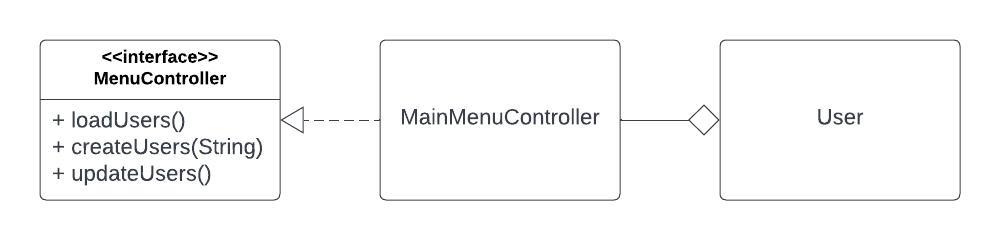
\includegraphics[scale=0.7] {img/users.png}
        \caption{Rappresentazione UML della gestione degli utenti all'interno del MenuController .}
        \label{img:users}
    \end{figure}

    \paragraph{User} Rappresentato dalla omonima classe rappresenta un utente che definisce la composizione degli utenti, questo model è estremamente rilevante in quanto contiene le informazioni necessarie che verranno caricate al momento del login.

    Pertanto, la prima difficolta è stata identificare un metodo per salvare e caricare correttamente i dati da un file esterno in modo che non venissero persi una volta usciti dall’applicazione.

    Per risolvere questo problema ho deciso di optare per un file di tipo json in quanto ottimo per salvare e caricare oggetti tramite l’utilizzo della libreria gson, oltre ad avere già una leggera conoscenza pregressa sull’utilizzo di questo tipo di file.

    inoltre, durante la progettazione si sono tenuti in considerazione una serie di possibili scenari in modo da gestirli correttamente evitando errori:

    In caso il file json dove vengono salvati gli utenti non venga trovato ne viene automaticamente generato uno.

    L’aggiunta di nuovi livelli viene correttamente gestita in modo che durante il caricamento degli utenti se viene a mancare un’informazione riguardante un nuovo livello aggiunto viene automaticamente inizializzato con un valore di default.

    E in fine il file viene salvato ad ogni modifica significativa in modo onde evitare la perdita di dati dovuta alla erronea chiusura dell’applicazione


    \subsubsection{View}

    \begin{figure}[H]
        \centering{}
        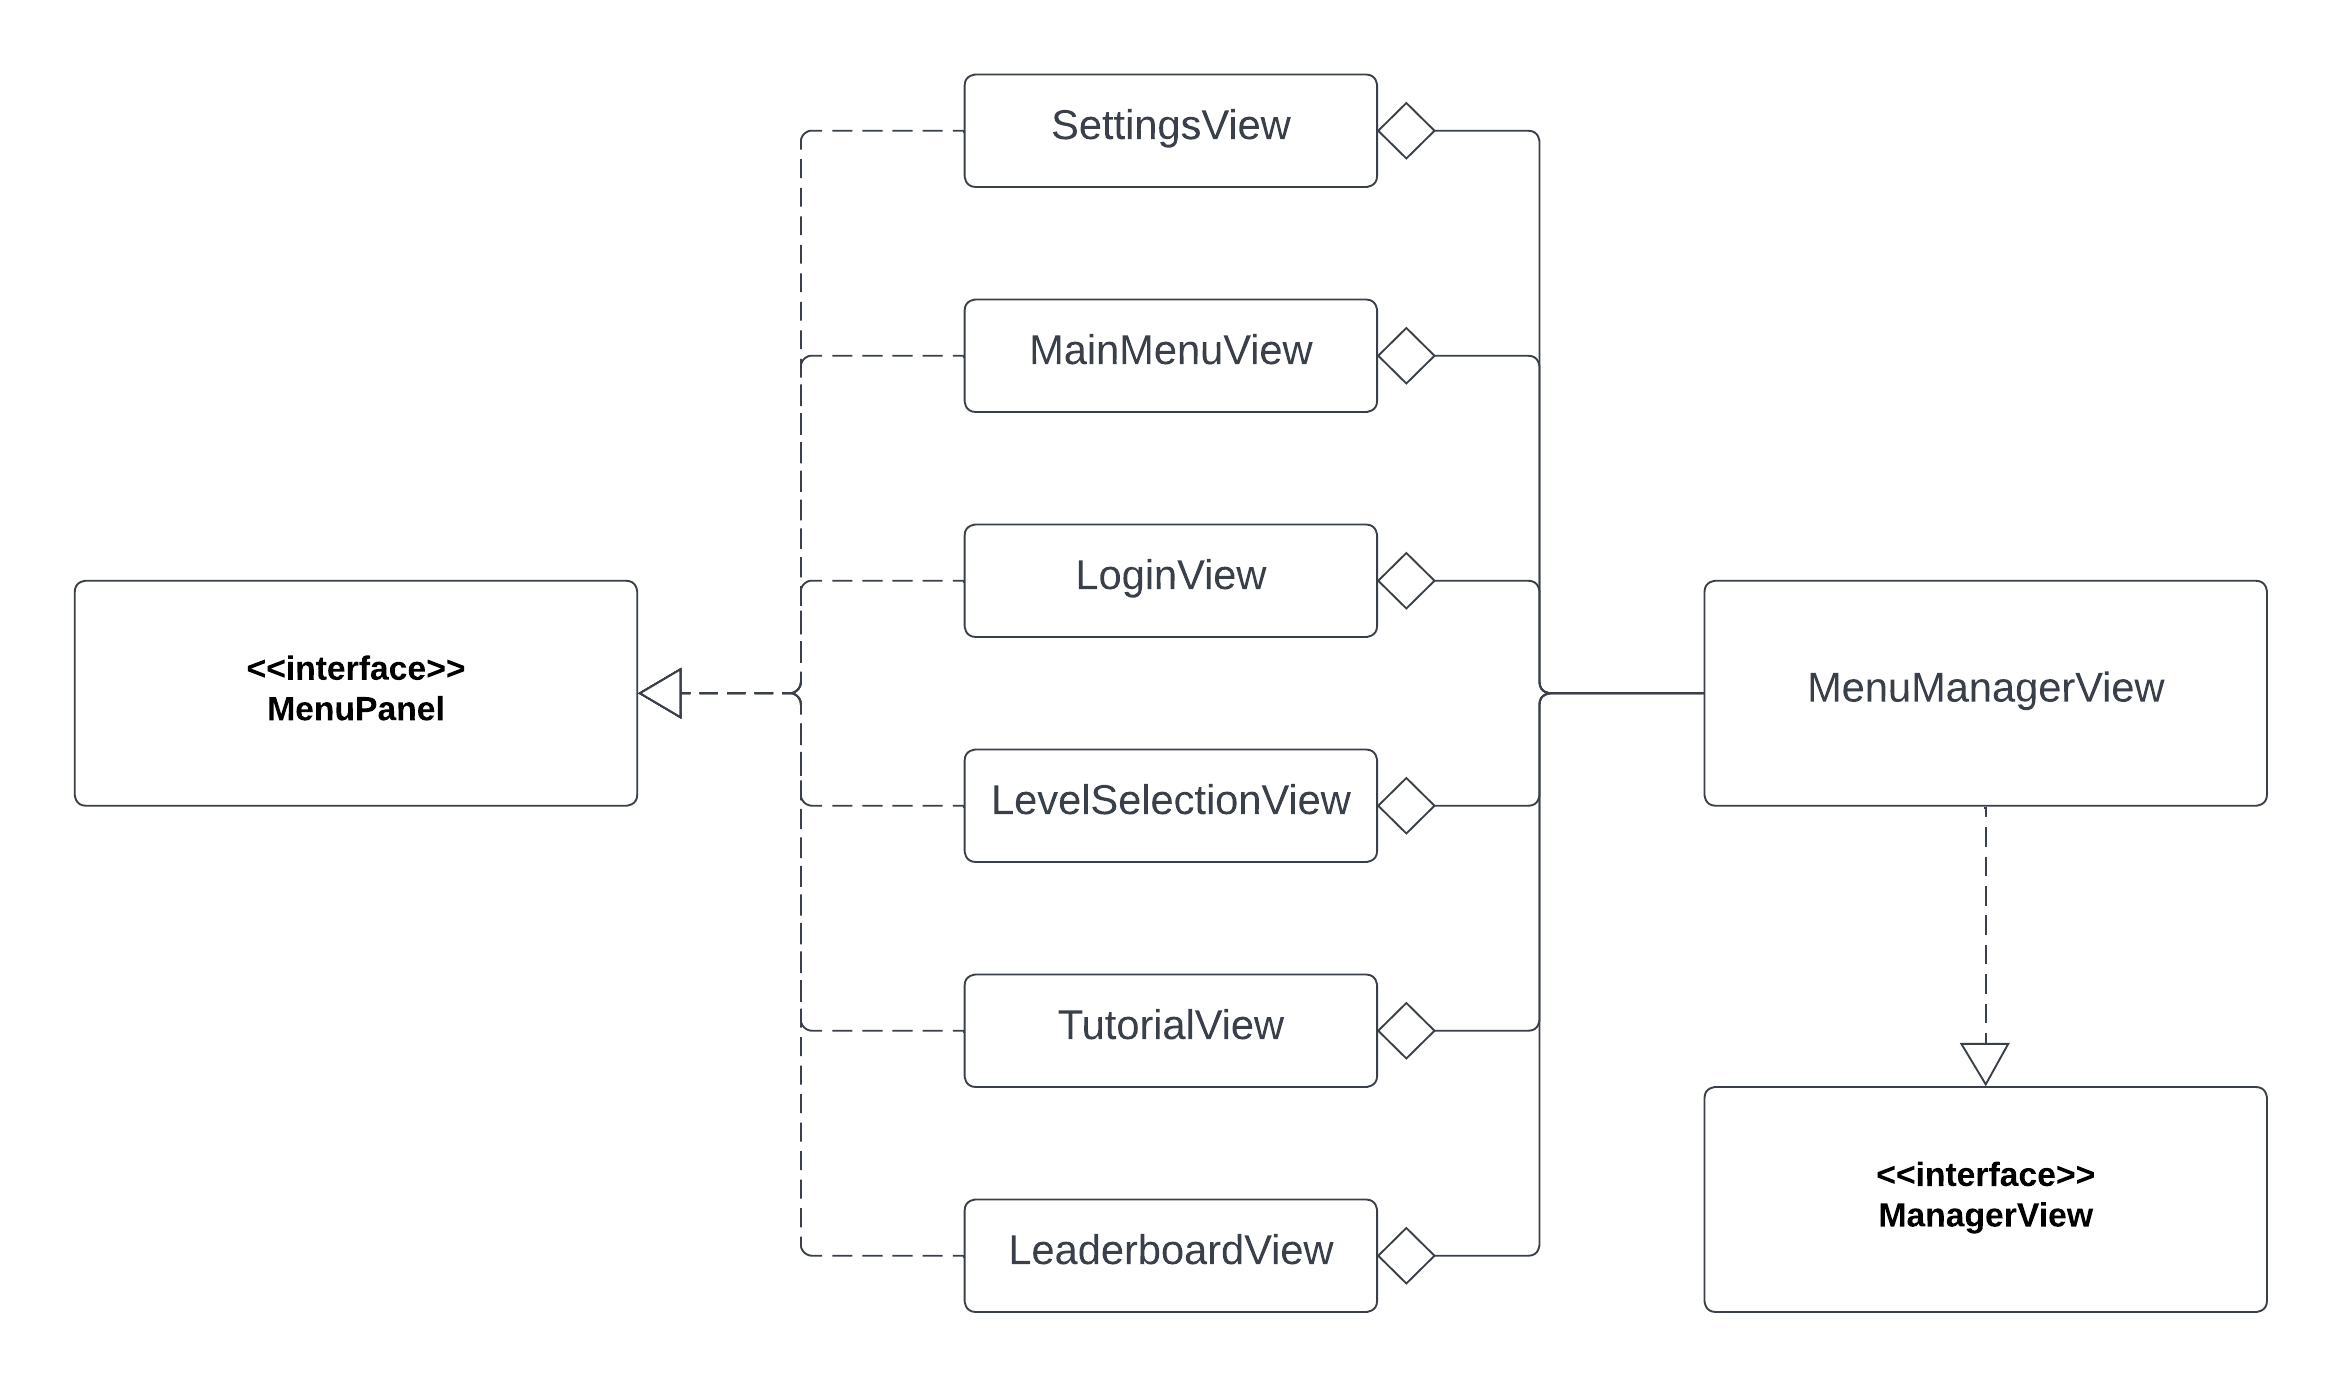
\includegraphics[scale=0.7] {img/view-manager.png}
        \caption{Rappresentazione UML della gestione dei pannelli della view.}
        \label{img:view-manager}
    \end{figure}

    \paragraph{ViewManager} Uno dei problemi principali nella parte view era quella di mostrare correttamente i diversi pannelli, in modo da evitare inutili ripetizioni e gestire in modo facile le varie view.

    per ovviare a questo problema si è optato per un manager che contenesse al suo interno i vari pannelli ed è rappresentata dalla classe MenuManagerView.

    Questa è un’implementazione della interfaccia ManagerView e si occupa della gestione delle view utilizzate nel menu principale, rappresenta il JFrame di tutta l’applicazione e gestisce il suo contenuto tra le diverse view presenti nel menu principale tramite le chiamate effettuate dal controller oltre a contenere elementi condivisi tra le diverse implementazioni di MenuPanel come animazioni, bottoni e scritte.

    \paragraph{MenuPanel} Questa interfaccainterfaccia identifica e definisce tutti i pannelli che la implementano dado loro semplici funzioni di base quale load e update

    \paragraph{Interfaccia utente customizzata} Una grande parte del mio contributo dal punto di vista visuale e funzionale viene dalla completa customizzazione dei vari Jcomponents con classi come CustomButton e CustomCheckBox e molte altre allo scopo di poter personalizzare aspetto in modo da essere più accattivante e di poter cambiare ogni propietàproprietà del component in sé per adattarlo all’utilizzo necessario, questo è specialmente marcato nelle sottoclassi di CustomButton che rappresentano tutti i vari tipi ed utilizzi di bottoni all’interno dei vari menu tutti posizionati usando coordinate relative alla grandezza dello schermo in frazioni per poter assicurare una facile scalabilità.

    \subsubsection{Controller}

    \begin{figure}[H]
        \centering{}
        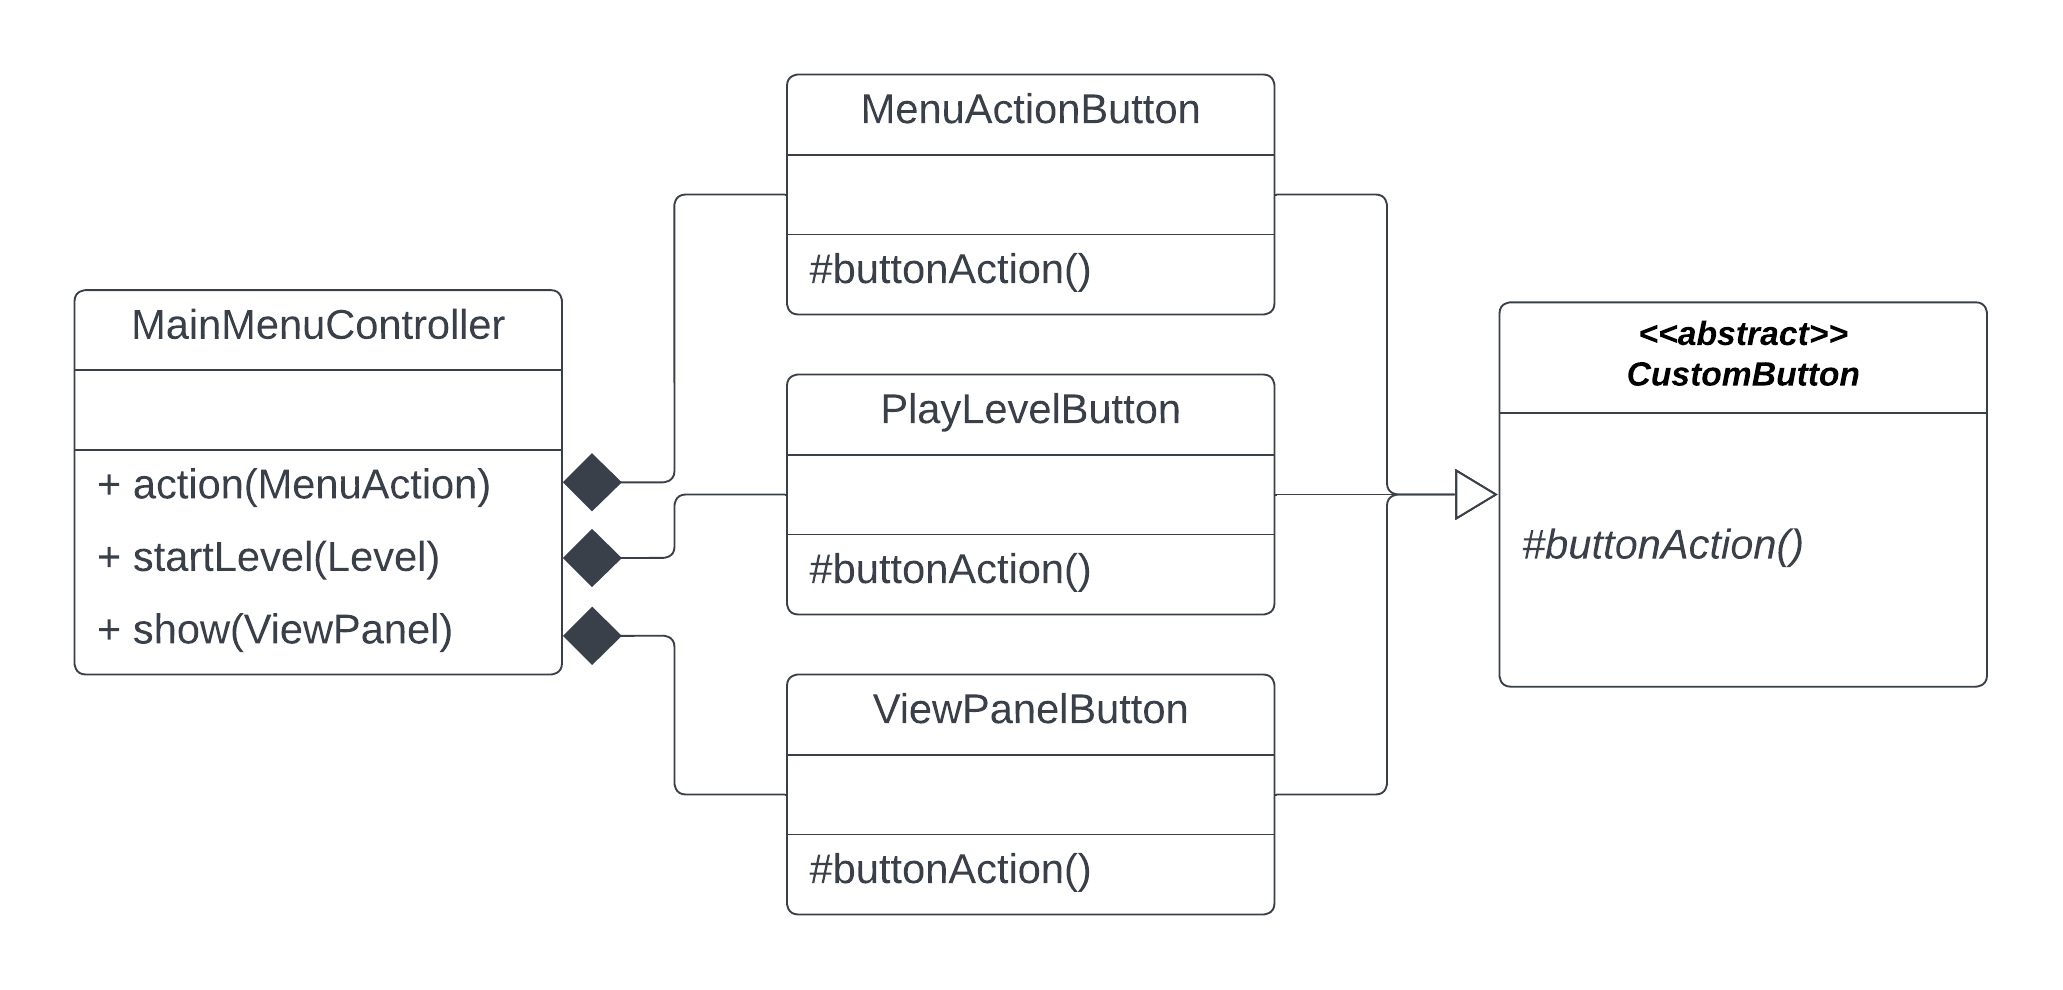
\includegraphics[scale=0.8] {img/menu-controller.png}
        \caption{Rappresentazione UML della classe MainMenuController.}
        \label{img:menu-controller}
    \end{figure}

    \paragraph{Il controller del menu principale} Per la gestione del menu principale ho deciso di optare per un unico controller che si occupasse di gestire ogni aspetto del menu principale, dalle azioni da eseguire dopo che uno specifico bottone è stato premuto all’aggiornamento del file dove vengono salvati gli utenti.

    Questo tipo di approccio è risultato molto efficace nella gestione delle impostazioni di gioco e del salvataggio degli utenti poiché direttamente relative al menu di gioco stesso e alle sue funzioni come il popolamento della leaderboard e la riproduzione di suoni e musiche.

    Oltre alla gestione di altre classi come l’aggiornamento degli utenti e delle dimensioni dello schermo.

    \subsubsection{I settings e i boost}

    Per finire mi sono anche occupato della gestione e modifica dei settings e dell’implementazione di boost (intesi come modificatori di statistiche del giocatore come velocità) all’interno del gioco, in questa parte la criticità più grande è  stataè stata fare in modo che lo schermo si adattasse in maniera corretta, controllata e automatica.

    Il problema era trovare un modo per far si che ogni componente fosse correttamente scalato e che l’utente non potesse erroneamente trovarsi in una situazione scomoda avendo una finestra più grande del proprio schermo.

    Per risolvere questo problema ho optato per una semplice risoluzione fissa con rateo 16:9 e una variabile che conteneva un’moltiplicatore che viene utilizzato da tutti i componenti visualizzati a schermo, controllando all’avvio dell’applicazione lo schermo in cui la finestra è aperta e mettendo la risoluzione più alta in 16:9 possibile senza uscire dai limiti dello schermo.

    Inoltre, un altro controllo fondamentale è stato quello di verificare che quando si prova a modificare la dimensione dello schermo la dimensione non ecceda i limiti dello schermo.

    Infine, questa impostazione insieme alle altre viene salvata all’interno del json in modo che venga caricato automaticamente al login.

    La creazione dei boost non ha portato nessuna particolare difficolta in quanto sono facilmente riuscito a riutilizzare il codice già creato in precedenza da Alam MD Shokot per entità con scopo simile modificando e aggiungendo le parti che mi interessavano e aggiungendo e modificando in parte l’implementazione del player

    \subsection*{Davide Valdifiori}

    In questa sezione l'attenzione è focalizzata sull'implementazione del livello di gioco col relativo caricamento della mappa da file e sul sistema  dei blocchi.

    \subsubsection{Livello}

    \begin{figure}[H]
        \centering{}
        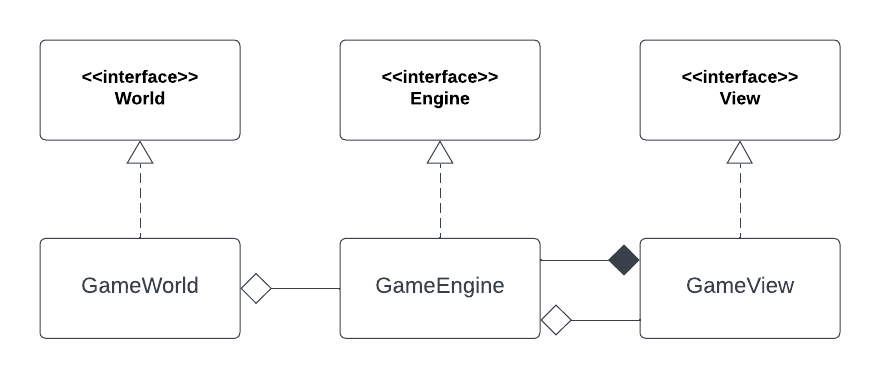
\includegraphics[scale=1] {img/livello-mvc.png}
        \caption{Rappresentazione UML del livello di gioco con le classi principali del pattern MVC e i rapporti fra loro.}
        \label{img:livello-mvc}
    \end{figure}

    \paragraph{Problema} Ciccio Pier ha più livelli di gioco, deve quindi essere possibile istanziare un nuovo livello partendo da un singolo parametro che lo identifica.

    \paragraph{Soluzione} Il sistema del livello di gioco utilizza il pattern MVC, come da Figura  \ref{img:livello-mvc}.
    E' formato dalle classi:

    \begin{itemize}
        \item \textbf{Model:} World - contiene gli oggetti del livello di gioco
        \item \textbf{Controller:} Engine - gestisce il livello e aggiorna gli elementi in gioco
        \item \textbf{View:} View - mostra a schermo il livello
    \end{itemize}

    \subsubsection{BlockFactory e EntityFactory}

    \begin{figure}[H]
        \centering{}
        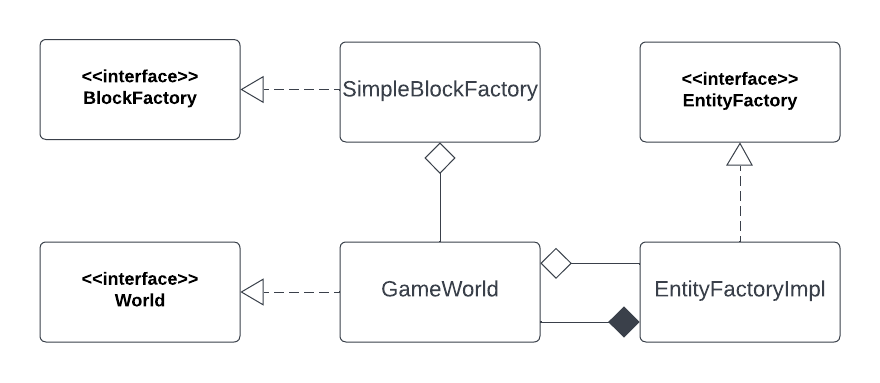
\includegraphics[scale=1] {img/world.png}
        \caption{Rappresentazione UML della classe GameWorld e delle factories.}
        \label{img:world}
    \end{figure}

    \paragraph{Problema} Durante la fase di implementazione ho trovato la necessità di implementare un metodo per creare nuove istanze di Block ed Entity partendo rispettivamente da BlockType ed EntityType, indipendentemente da quale implementazione delle interfacce venga usata.

    \paragraph{Soluzione} Ho deciso di utilizzare il factory method, come da Figura  \ref{img:world}, creando così due factories:
    \begin{itemize}
        \item \textbf{BlockFactory} contiene una unica funzione createBlock(BlockType type) per creare un nuovo \emph{Block} dato un \emph{BlockType}
        \item \textbf{EntityFactory} contiene le funzioni createPlayer() e createEntity(EntityType type) per creare rispettivamente il \emph{Player} e una nuova \emph{Entity} data una \emph{EntityType}
    \end{itemize}

    \subsubsection{WorldLoader}

    \begin{figure}[H]
        \centering{}
        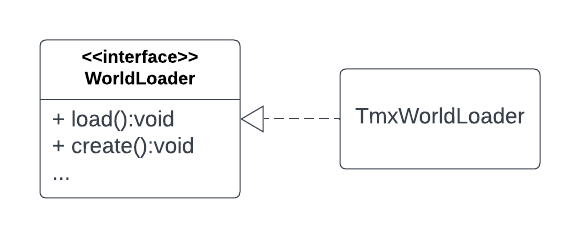
\includegraphics[scale=1] {img/worldloader.png}
        \caption{Rappresentazione UML del WorldLoader, con la sua implementazione TmxWorldLoader.}
        \label{img:worldloader}
    \end{figure}

    \paragraph{Problema} In fase di sviluppo è nata la necessità di creare un modo semplice per caricare i dati del livello di gioco da file.

    \paragraph{Soluzione} Dato in futuro potrebbe essere necessario poter cambiare tipologia di file, ho optato per la creazione di una interface \emph{WorldLoader}, come visibile in Figura \ref{img:worldloader}.

    WorldLoader è stata creata con lo scopo di rendere semplice la creazione di una nuova implementazione che possa popolare un oggetto World da altri tipi di files con estensioni e formati differenti.

    La classe \emph{TmxWorldLoader} è l'implementazione dell'interfaccia WorldLoader. Ha lo scopo di caricare tutte le informazioni da un file con estensione \emph{.tmx}, il costruttore ha come parametri il nome del file e una istanza di World.

    \subsubsection{View del Livello}

    \begin{figure}[H]
        \centering{}
        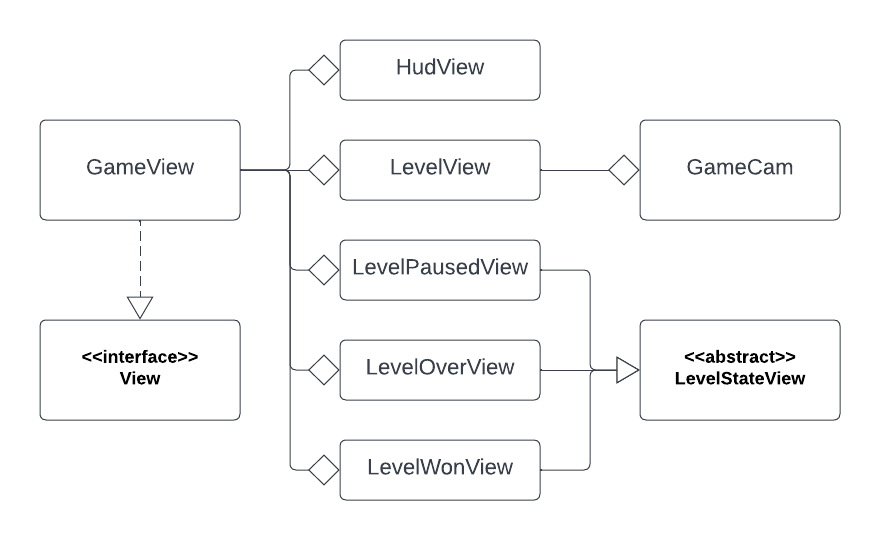
\includegraphics[scale=0.8] {img/view.png}
        \caption{Rappresentazione UML della classe GameView.}
        \label{img:view}
    \end{figure}

    \paragraph{Problema} Rappresentare a schermo il livello di gioco e sovrapporre la visualizzazione di schermate di pausa, vittoria, sconfitta.

    \paragraph{Soluzione} Utilizzo di una classe GameView che estende JLayeredPane, permettendo così di inserire pannelli sovrapposti. Come visibile in Figura \ref{img:view}, è composta da:

    \begin{itemize}
        \item \textbf{LevelView}: viene utilizzato per mostrare a schermo tutti gli oggetti di gioco presenti in World. Al suo interno contiene una istanza di \emph{GameCam}, che viene utilizzata per calcolare quale area del mondo mostrare a schermo, centrando la visuale sulla posizione corrente del Player
        \item \textbf{HudView}: viene utilizzato per mostrare le barre di vita e stamina, le monete e il punteggio del giocatore
        \item \textbf{LevelPausedView}: viene mostrato solo quando il gioco è in pausa
        \item \textbf{LevelOverView}: viene mostrato solo quando il giocatore muore e perde il gioco
        \item \textbf{LevelWonView}: viene mostrato solo quando il giocatore arriva alla fine del livello e vince il gioco
    \end{itemize}

    \subsubsection{Blocchi}

    \begin{figure}[H]
        \centering{}
        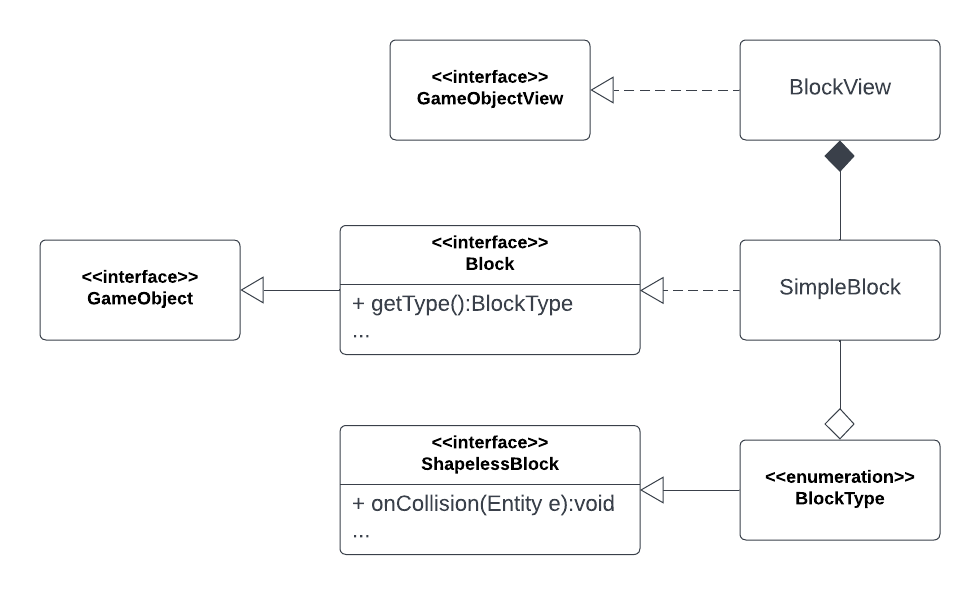
\includegraphics[scale=0.8] {img/block.png}
        \caption{Rappresentazione UML delle interface Block e BlockView, con le loro relative implementazioni e classi associate.}
        \label{img:block}
    \end{figure}

    \paragraph{Problema} Ogni livello è composto da dei blocchi fisici o decorativi che devono essere rappresentati in gioco.

    \paragraph{Soluzione} I blocchi non utilizzano il pattern MVC, poichè non devono svolgere nessuna manipolazione sul Model e il Controller diverrebbe inutile.
    Per ridurre il numero di classi istanziate ho optato per una soluzione in cui esso non è presente, quindi si ha solo l'interface \emph{Block} che estende \emph{GameObject}, come visibile in Figura \ref{img:block}.
    Estendendo GameObject si dovrà quindi fornire anche una istanza di \emph{GameObjectView} quando viene chiamata la funzione getView(), a cui verrà delegato il compito di mostrare a schermo il blocco.

    \subsubsection{Block Model}

    Anche per i blocchi è presente una enumerazione \emph{BlockType} che ne definisce la tipologia e altre proprietà generiche per quel tipo di blocco.

    La classe \emph{SimpleBlock} è l'implementazione dell'interfaccia Block, il suo costruttore ha come parametro BlockType.

    E' presente anche una interface ShapelessBlock che rappresenta i blocchi non solidi con cui si può interagire, permette di eseguire una azione nel momento in cui il giocatore lo attraversa.

    \subsubsection{Block View}

    La classe BlockView è l'implementazione dell'interfaccia GameObjectView, si occupa di rappresentare a schermo un blocco.

    \subsection*{Riccardo Mingozzi}

    \subsubsection{Entità generali}

    \begin{figure}[H]
        \centering{}
        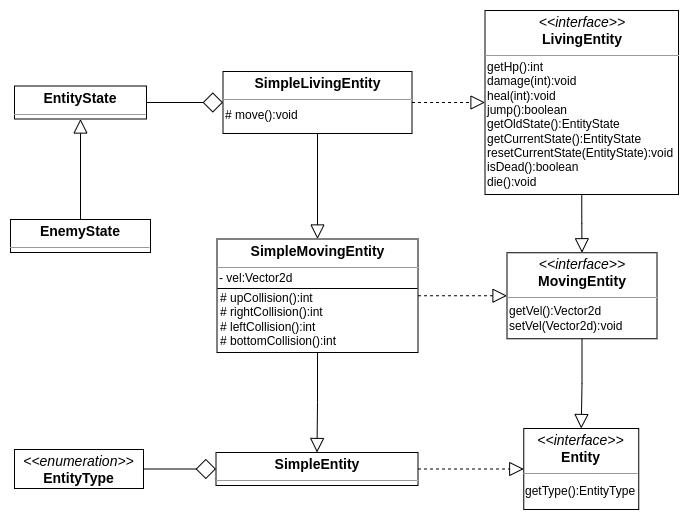
\includegraphics[scale=0.5] {img/entities-general.png}
        \caption{Rappresentazione UML della struttura delle classi base delle entità.}
        \label{img:entities-general}
    \end{figure}

    \paragraph{Problema} Trovare un modo di unificare e generalizzare la rappresentazione di tutte le entità, riuscendo ad astrarre i loro aspetti distintivi principali, permettendo una facile e permissiva estensione o aggiunta di ulteriori entità

    \paragraph{Soluzione} Ideazione di una gerarchia, consistente in una distinzione tra entità statiche, semoventi e viventi.

    La base di questa gerarchia sono infatti le entità statiche, che in composizione con una enumerazione rappresentate tutte le entità, permette di avere un riferimento ad informazioni comuni a tutte, quali larghezza, altezza, eventuale vita ed eventuale danno, senza dover salvare queste informazioni in ogni classe individuale.

    Le entità semoventi presentano invece un Vector2d aggiuntivo (oltre quello della posizione attuale) rappresentate la sua accelerazione e vari metodi per controllare le collisioni.

    La classe infine delle entità viventi presenta campi e metodi per gestire i loro punti vita, metodi per gestire il movimento (salto incluso)  tenendo conto di eventuali collisioni, oltre che possedere degli stati, rappresentati dalla composizione con enumerazione. Da quest’ultima classe di entità sono poi state derivate le classi del player e dei nemici.

    \subsubsection{Nemici}

    \begin{figure}[H]
        \centering{}
        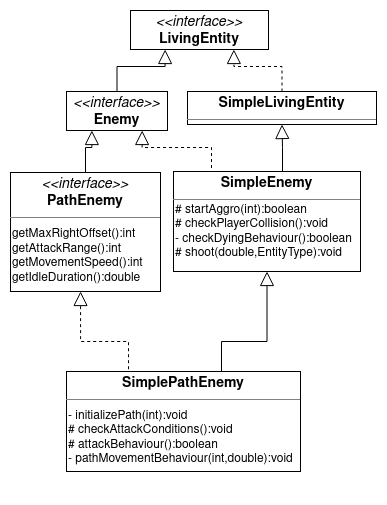
\includegraphics[scale=0.7] {img/enemies.png}
        \caption{Rappresentazione UML della gestione dei nemici.}
        \label{img:enemies}
    \end{figure}

    \paragraph{Problema} Trovare un’astrazione rappresentate i nemici, generica e flessibile tale che permetta facilmente di aggiungere nuovi nemici, riducendo gli elementi distintivi da implementare di ogni nemico al minimo.

    \paragraph{Soluzione} Inizialmente creata una sola classe per i nemici, dove si sono astratti i controlli di morte e di collisione con il player, identici per tutti i nemici.

    Successivamente questa classe è stata estesa in un’altra sempre generica, rappresentate la tipologia di nemico più comunemente diffuso nei platform 2D, ossia quello che pattuglia un segmento di mappa, attaccando il nemico solo quando in range.

    Questo comportamento è stato dunque astratto, generalizzando il movimento, prendendo solo la lunghezza del segmento e la velocità da parametri individuali per ogni nemici, utilizzando invece un template method per l’attacco. Per quest’ultimo, il template consiste nel chiamare un metodo quando il nemico soddisfa le condizione per iniziare l’attacco ed un altro quando invece non attacca, entrambi poi implementati in modo singolo per ogni nemico.

    \subsubsection{Proiettili}

    \begin{figure}[H]
        \centering{}
        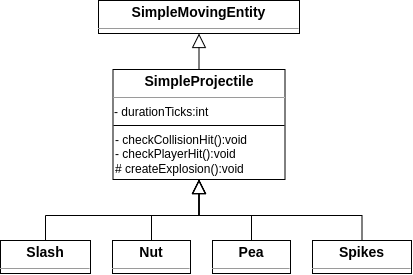
\includegraphics[scale=0.6] {img/projectiles.png}
        \caption{Rappresentazione UML dei proiettili e delle relative sottoclassi.}
        \label{img:projectiles}
    \end{figure}

    \paragraph{Problema} Riuscire a rappresentare i proiettili in modo efficiente permettendo un’estrema facilità di aggiunta

    \paragraph{Soluzione} Creazione di una classe astratta per i proiettili, estendendo tutto il comportamento, principalmente il movimento, permettendo che l’aggiunta di nuovi proiettili richieda, in caso seguano il comportamento comune individuato, solo poche informazioni individuali, quali velocità di movimento e durata.

    \subsection*{MD Shokot Alam}

    \subsubsection{Gestione rappresentazione del movimento}

    \begin{figure}[H]
        \centering{}
        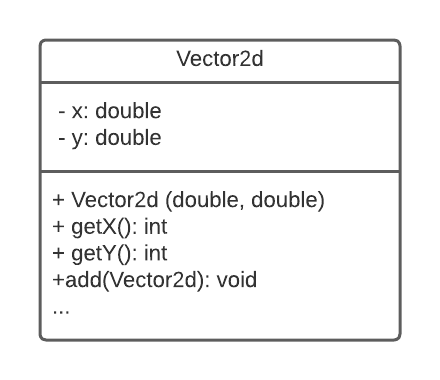
\includegraphics[scale=0.75] {img/vector.png}
        \caption{Rappresentazione UML della classe Vector2d.}
        \label{img:vector}
    \end{figure}

    In fase di sviluppo si presenta  il problema della gestione del sistema di movimento di qualsiasi entità vivente o non nella finestra di gioco.

    Ho dunque proceduto alla creazione di una  classe ausiliaria Vector2d preposta  al supporto delle altre  entità per il posizionamento e metodi adibiti allo spostamento.

    \subsubsection{Gestione Item}

    \begin{figure}[H]
        \centering{}
        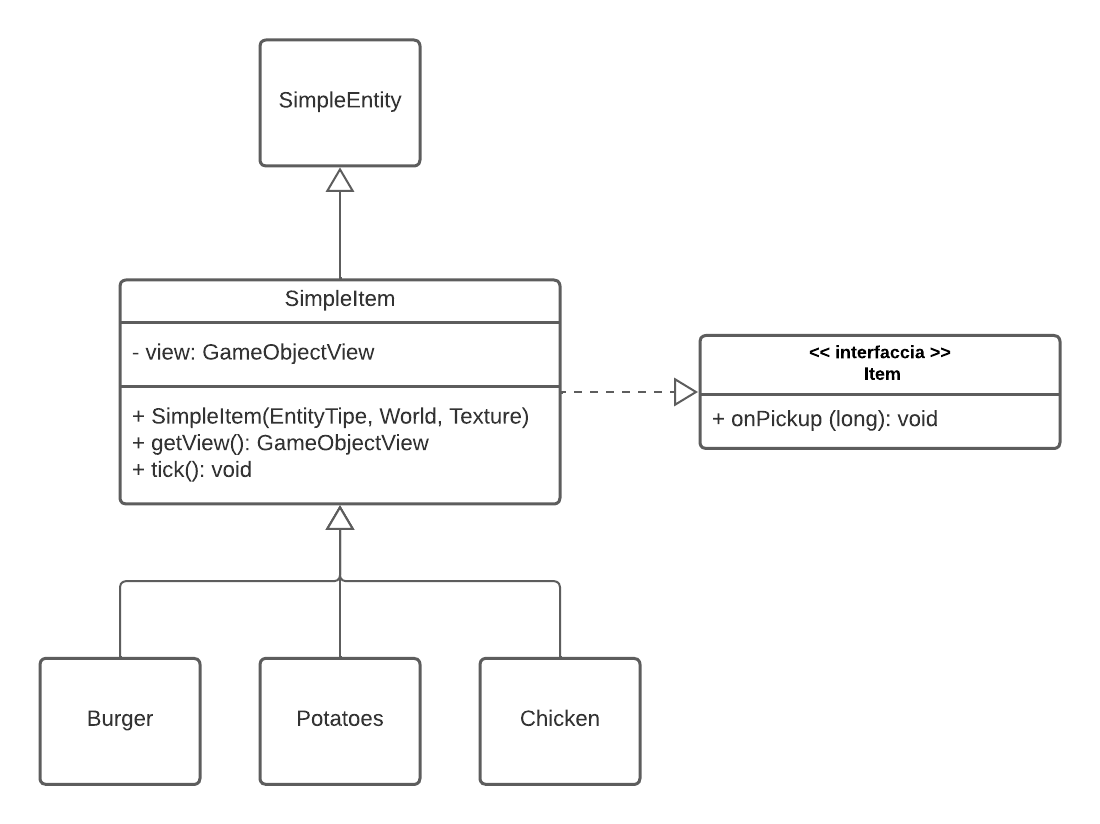
\includegraphics[scale=0.75] {img/simple-item.png}
        \caption{Rappresentazione UML della classe SimpleItem e relative estensioni.}
        \label{img:simple-item}
    \end{figure}

    La rappresentazione dei vari oggetti es: Potatoes, Burger e i  vari potenziamenti ha costituito un problema di duplicazione del codice, per questo ho creato una classe SimpleItem che generalizza le loro funzionalità comuni e ciò  ha dato seguito alla realizzazione di una classe analoga per la renderizzazione.

    \subsubsection{Gestione animation}

    All'inizio si era manifestata la problematica della diversificazione rappresentativa delle view. Per unificare i vari modi di rappresentazione ho creato la classe Animation.

    \subsubsection{Gestione suoni}

    \begin{figure}[H]
        \centering{}
        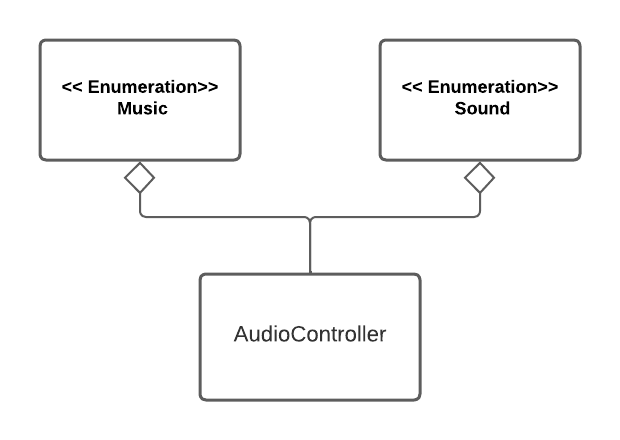
\includegraphics[scale=1] {img/audio.png}
        \caption{Rappresentazione UML della classe AudioController e delle enumerazioni Sound e Music.}
        \label{img:audio}
    \end{figure}

    Per la gestione dei suoni ho creato due enumerazioni Music e Sound, una per il controllo della musica e l'altra  per gli effetti sonori.

    In entrambi ho utilizzato la classe Clip fornito da javax.sound.sampled, che mi permette la riproduzione di un qualsiasi suono in formato wav.

    Successivamente ho realizzato la classe AudioController per la gestione del volume e la  riproduzioni dei vari suoni.

    \subsubsection{Gestione Boss}

    \begin{figure}[H]
        \centering{}
        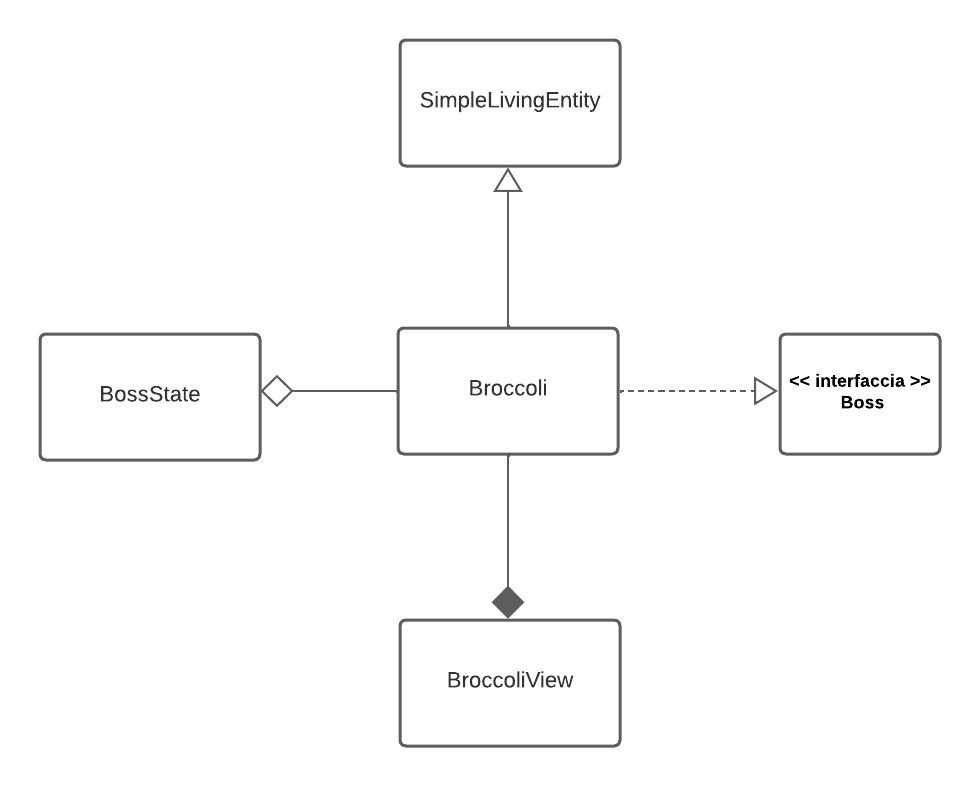
\includegraphics[scale=1] {img/boss.png}
        \caption{Rappresentazione UML della classe Broccoli.}
        \label{img:boss}
    \end{figure}

    In fase di analisi ho realizzato un nemico che ha più stati, i più importanti sono: lo stato di inseguimento del player e i tre stati dell'attacco.

    Per gli attacchi ho cercato di differenziarli tra:

    \begin{itemize}
        \item lancio di missili ad inseguimento
        \item caduta di meteore
        \item spara raggio laser
    \end{itemize}

    \subsubsection{Gestione SimpleEntityView}

    \begin{figure}[H]
        \centering{}
        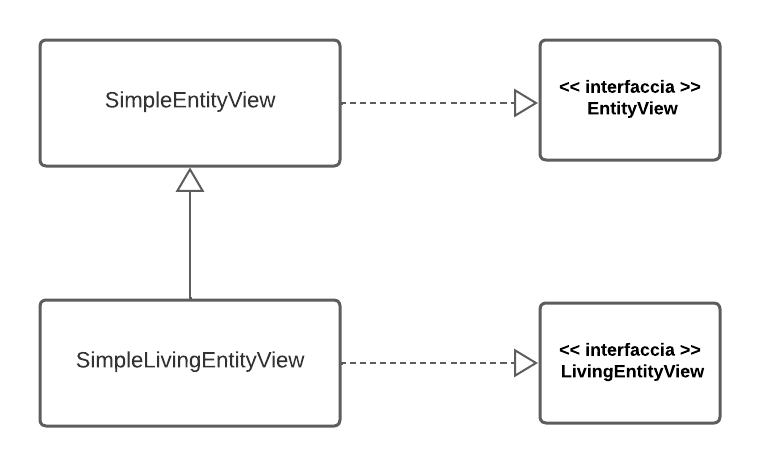
\includegraphics[scale=1] {img/entities-view.png}
        \caption{Rappresentazione UML delle classi SimpleEntityView e SimpleLivingEntityView.}
        \label{img:entities-view}
    \end{figure}

    In fase di analisi si è presentata la medesima casistica degli item ma in questo caso in rapporto all'entità. ho proceduto alla riunificazione dei vari tipi di entità quali:

    \begin{itemize}
        \item SimpleEntityView
        \item SimpleLivingEntityView
    \end{itemize}

    \chapter{Sviluppo}

    \section{Testing automatizzato}

    Le problematiche più complesse erano riscontrabili solo in casi limite molto difficili da ricreare in un ambiente automatizzato, per questo abbiamo optato per una verifica manuale del corretto funzionamento di alcune funzionalità del gioco, come per esempio le collisioni delle entità coi blocchi.

    Dato che alcuni di noi han programmato e testato su Linux e Mac durante tutta la durata del progetto, siamo sempre riusciti a controllare subito se una funzionalità o una porzione di codice non funzionava sui principali sistemi operativi.

    Ognuno di noi ha creato alcuni test in JUnit per testare alcune funzionalità della propria area di progetto:
    \begin{itemize}
        \item \textbf{BoostTest:} funzionamento di tutti i boost quando vengono raccolti dal player
        \item \textbf{BossTest:} spawn e cambio di stato del boss
        \item \textbf{EnemiesTest:} spawn e cambio di stato dei nemici e attacco del player
        \item \textbf{GameWorldTest:} gran parte delle funzionalità della classe GameWorld
        \item \textbf{PlayerTest:} punteggio, vita e stamina del player
        \item \textbf{TmxWorldLoaderTest:} caricamento degli elementi di gioco da file tmx
        \item \textbf{UsersTest:} caricamento e salvataggio degli utenti da file json
    \end{itemize}

    \section{Metodologia di lavoro}

    La fase di analisi e fase di design architetturale sono state svolte in gruppo. Nel corso della realizzazione del progetto, ci siamo periodicamente incontrati virtualmente sulla piattaforma Discord per discutere delle scelte implementative ed aiutarci reciprocamente nel caso di dubbi.

    Tuttavia è capitato in alcuni casi che il design progettato non sia stato rispettato perché uno o più componenti del gruppo han trovato una soluzione migliore per realizzare alcune parti del progetto di loro competenza, che han poi portato a volte alla necessità di applicare modifiche ad altre parti. In questi casi si è sempre concordato e comunicato come applicare le modifiche agli altri membri.

    Nonostante tutto, la divisione iniziale dei lavori e delle parti è stata rispettata e possiamo affermare che anche la suddivisione dei ruoli è stata equilibrata. Le parti che
    ciascuno di noi ha sviluppato si sono rivelate essere in alcuni casi leggermente dipendenti fra loro, ma siamo comunque riusciti a portare a termine il progetto senza ostacolarci a vicenda accordandoci in fase di design comune.

    Come specificato nella sezione di design dettagliato, qui di seguito la
    suddivisione dei compiti che ciascun componente ha svolto:

    \subsubsection{Alessandro Aldini}

    \begin{itemize}
        \item Creazione di JComponent personalizzati
        \item Gestione base di model, view e controller del menu principale
        \item Gestione impostazioni di volume di gioco
        \item Gestione leaderboard di gioco
        \item Gestione risoluzione e ridimensionamento dello schermo
        \item Gestione di creazione e modifica degli utenti
        \item Implementazione di boosts
    \end{itemize}

    Durante lo sviluppo il mio metodo di programmazione è stato quello di cercare di avere subito delle calassi seppur grezze funzionanti, in modo da poter avere una visione di insieme e un’idea su come riuscivo a gestire i tempi.

    E successivamente migliorare e perfezionare le classi o il loro funzionamento in modo da rendere il codice più pulito e corretto, questo metodo è stato molto efficace per me perché durante lo sviluppo riuscivo a notare i punti che erano migliorabili e a modificarli nel tempo, arrivando ad un risultato di cui mi sento soddisfatto.

    Inoltre, ho cercato sempre di pensare all’espandibilità del mio codice facendo sì che sia facilmente modificabile, sfortunatamente per via di mancanza di tempo disponibile al progetto rimangono alcune enum che sarebbero dovute diventare classi per poterle rendere perfettamente espandibili.

    La parte di integrazione fra GameEngine e MainMenuController `e stata
    sviluppata in collaborazione con Davide Valdifiori.

    La parte di implementazione dei boost è stata sviluppata in collaborazione con Alam MD Shokot
    \subsubsection{Davide Valdifiori}

    \begin{itemize}
        \item Gestione base di Model, View e Controller del livello
        \item Caricamento della mappa da file
        \item Gestione dei blocchi
        \item Gestione dell'input da tastiera e controller
        \item Loop del gioco
    \end{itemize}

    La parte di integrazione fra GameEngine e MainMenuController è stata sviluppata in collaborazione con Alessandro Aldini.

    \subsubsection{Riccardo Mingozzi}

    \begin{itemize}
        \item Struttura base delle entità
        \item Struttra base del player e  attacco
        \item View (inzialmente) e Model di tutti i Nemici
    \end{itemize}

    Avevo inizialmente creato un sistema per gestire la view dei nemici, basato su degli stati che venivano aggiornati nel model, in quanto usati per determinare i loro
    comportamenti.

    In fase di analisi avevamo ritenuto corretto dividere le view di nemici, player e boss, in quanto molto diversi come comportamenti. Successivamente abbiamo deciso di astrarre le varie view, estendendo il concetto di rappresentazione basata su stati a tutte le entità.

    Questa parte è stata poi implementata dal mio collega MD Shokot Alam.

    \subsubsection{MD Shokot Alam}

    \begin{itemize}
        \item Sviluppo del boss
        \item Cibi grassi
        \item Sistema delle monete
        \item Sistema della stamina e della vita del player
        \item Collisioni delle entità
        \item Sistema di movimento delle entità
        \item View base e animazioni delle entità
        \item Sistema di suoni e musica del gioco
    \end{itemize}

    Per la realizzazione del sistema audio ho riscontrato problemi per la riproduzione di suoni su sistemi Linux, per risolvere questo problema, ho trovato la soluzione su StackOverflow. Ho poi adattato il codice alle mie esigenze.

    \section{Note di sviluppo}

    \subsubsection{Alessandro Aldini}

    Features avanzate utilizzate:

    \begin{itemize}
        \item Uso di lambda expressions
        \item Uso di Stream, Optional e altri costrutti funzionali
        \item Uso di librerie di terze parti:
        \begin{itemize}
            \item \href{https://github.com/google/gson}{Gson} per caricare e salvare gli utenti su un file json
            \item \href{https://github.com/qos-ch/slf4j}{SLF4J} logger
        \end{itemize}
    \end{itemize}

    \subsubsection{Davide Valdifiori}

    Features avanzate utilizzate:

    \begin{itemize}
        \item Creazione classe Pair$<$T$>$
        \item Uso di lambda expressions
        \item Uso di Stream, Optional e altri costrutti funzionali
        \item Uso di librerie di terze parti:
        \begin{itemize}
            \item \href{https://github.com/csueiras/libtiled-java}{Libtiled} per caricare la mappa da files tmx
            \item \href{https://github.com/williamahartman/Jamepad}{Jamepad} per gestire l'input da Controllers
            \item \href{https://github.com/qos-ch/slf4j}{SLF4J} logger
        \end{itemize}
    \end{itemize}

    \subsubsection{Riccardo Mingozzi}

    Features avanzate utilizzate:

    \begin{itemize}
        \item Uso di lambda
        \item Uso di Stream, Optional e altri costrutti funzionali
        \item Sviluppo di algoritmo di attacco del player: un metodo che filtra selettivamente le entità in range, facendo gli appositi controlli, attaccando il nemico più vicino che rispetti le condizioni di attacco
    \end{itemize}

    \subsubsection{MD Shokot Alam}

    Features avanzate utilizzate:

    \begin{itemize}
        \item Uso di Optional e altri costrutti funzionali
        \item Uso di parti di libreria non spiegate a lezione:
        \begin{itemize}
            \item javax.sound.sampled per gestire i suoni e le musiche di gioco
        \end{itemize}
    \end{itemize}

    \chapter{Commenti finali}

    \section{Autovalutazione e lavori futuri}

    \subsubsection{Alessandro Aldini}

    Alla fine di questo progetto mi ritengo estremamente soddisfatto del mio lavoro e di questo progetto in generale.

    Sono contento del metodo di lavoro che ho deciso di seguire durante questo progetto e sono orgoglioso del mio lavoro considerando le mie conoscenze pregresse e le svariate conoscenze acquisite durante tutta la fase di sviluppo; ma soprattutto sono davvero fiero del risultato finale, tenendo conto che nessuno di noi aveva mai fatto qualcosa di simile e che si tratta comunque di un progetto universitario penso che il prodotto finale sia davvero curato nei dettagli e appassionato.

    Penso, inoltre, che ci sia stato un ottimo team work in quanto si era sempre disponibili per confronti e aiuti durante la parte di sviluppo nei confronti di tutti così da evitare possibili problemi e ritardi durante questa parte.

    Durante lo sviluppo una pecca che ho notato verso la fine è stata l’aggiunta di JavaDoc dopo aver già pushato le funzioni e classi, questo è dovuto al fatto che spesso si lavorava insieme e si comunicavano i cambiamenti quindi non sentivo che questa parte fosse fondamentale ma mi rendo conto che in un ambiente di lavoro questa rappresenta una mancanza importante e ne ho preso atto.

    Sarei interessato nel futuro a proseguire la creazione di questo progetto, portandolo anche nel mondo mobile.

    \subsubsection{Davide Valdifiori}

    Sono abbastanza soddisfatto di come ho sviluppato la mia parte del progetto e del risultato finale.

    Avendo già conoscenze pregresse in Java sono riuscito a portare avanti la mia parte di progetto senza troppe difficoltà, ma sono comunque riuscito a imparare molto da questa esperienza, soprattutto grazie alla collaborazione dei miei compagni di progetto e alle loro idee.

    Questo progetto mi ha insegnato le basi del lavoro di gruppo e tanto altro che da solo non avrei potuto imparare, quindi nel complesso valuto questa esperienza positivamente.

    Sarei interessato nel futuro a proseguire la creazione di questo progetto, portandolo anche nel mondo mobile.

    \subsubsection{Riccardo Mingozzi}

    Considerando come questo sia stato il mio primo approccio al game development, al teamworking, allo sviluppo di un progetto complesso ed articolato, non sono totalmente insoddisfatto del mio risultato.

    Riconosco tuttavia che tutto il mio lavoro poteva essere fatto molto meglio, ed infatti questo progetto mi ha illuminato sulle lacune che devo affrontare per approcciarmi a futuri progetti di questa complessità.

    Mi ha inoltre insegnato tanto relativamente il lavoro di gruppo, permettendomi di sviluppare parallelamente tante soft skills che sicuramente torneranno utili in futuro.

    \subsubsection{MD Shokot Alam}

    Sono molto soddisfatto del progetto eseguito e felice  di averlo portato a termine.

    L'obiettivo principale  che mi ero prefissato era creare un nemico univoco che si autogestisca in base allo stato in cui si trova con un codice pulito e più comprensibile possibile. A causa della mia inesperienza ho dovuto però spesso ristrutturare il codice per eliminare duplicazioni e facilità di utilizzo.

    Nel complesso valuto questa esperienza molto positivamente in quanto ha permesso di lavorare in team, una soft skill importate nell'ambito lavorativo.

    In futuro vorrei creare altri progetti, anche in settori diversi dall'ambiente gaming.

    \appendix
    \chapter{Guida utente}

    \begin{figure}[H]
        \centering{}
        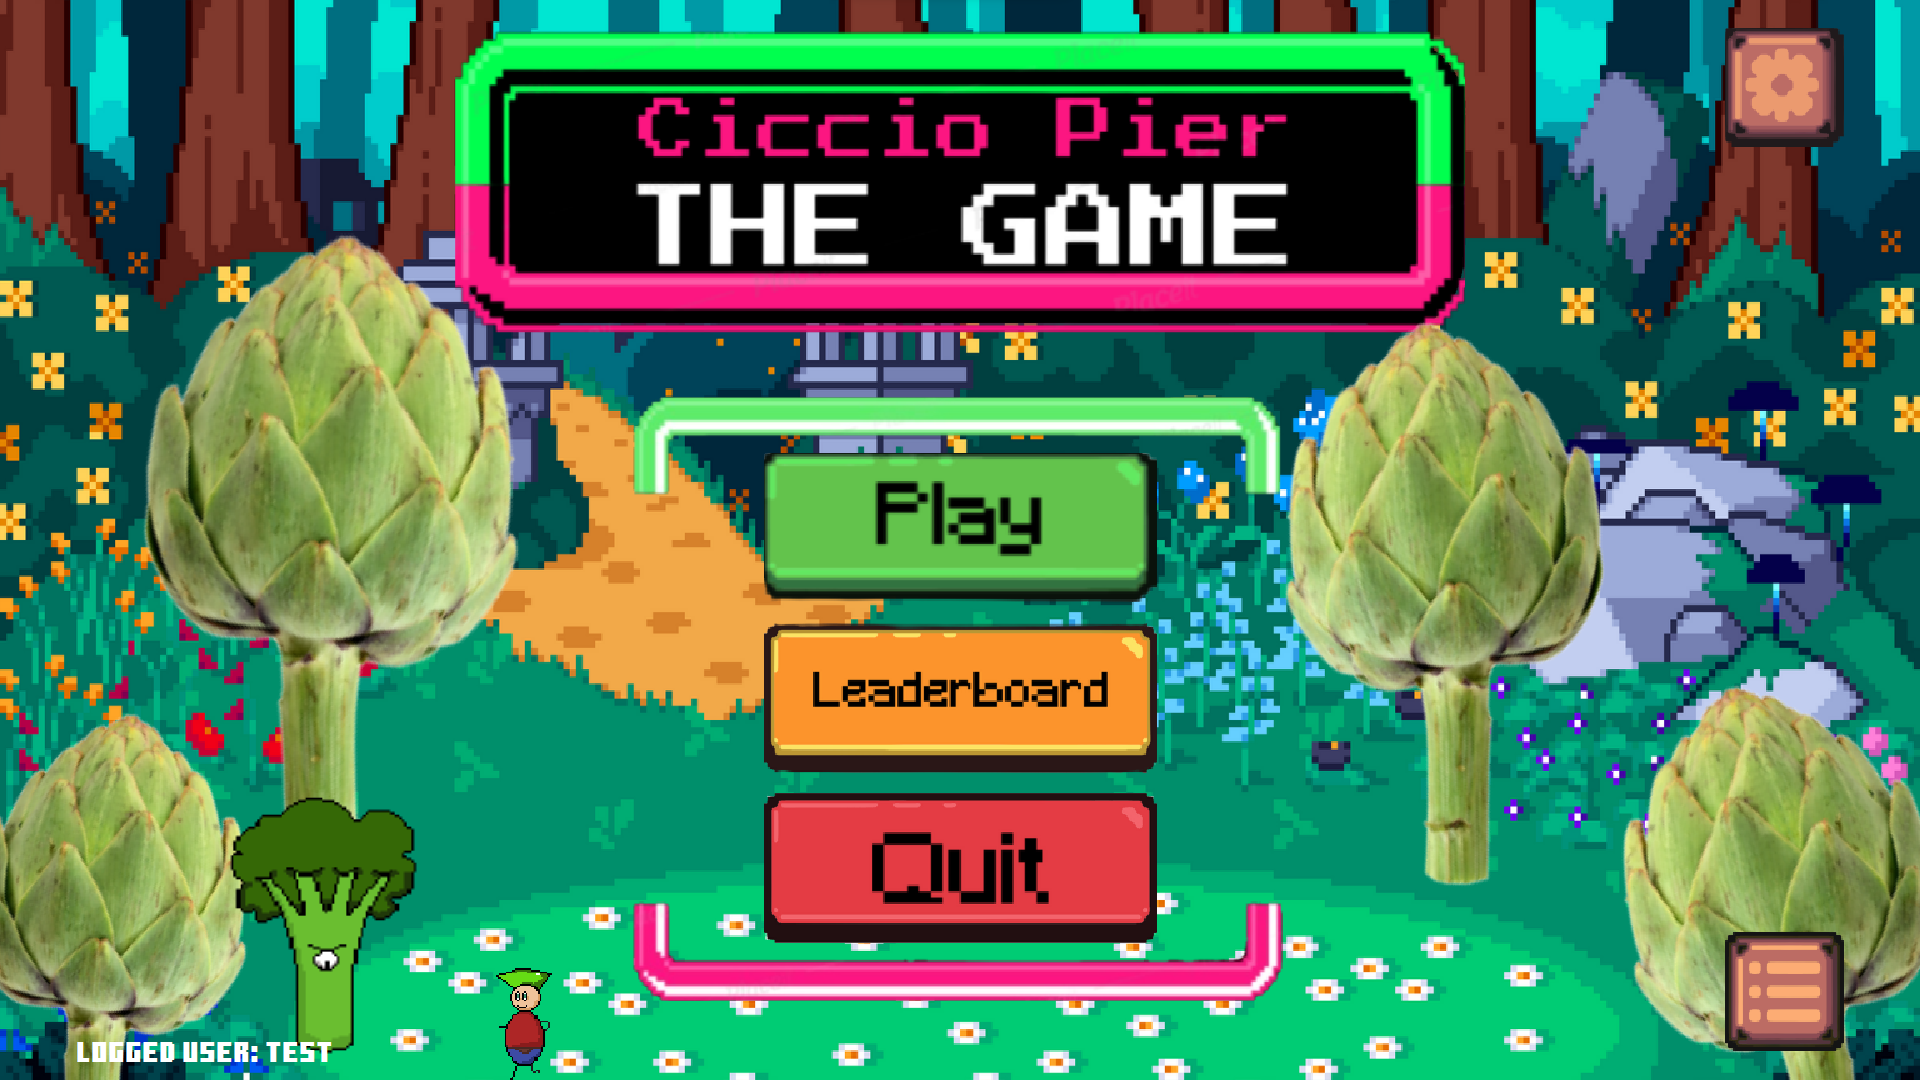
\includegraphics[scale=0.2] {img/game-menu.png}
        \caption{Schermata iniziale del gioco.}
        \label{img:game-menu}
    \end{figure}

    Quando si apre il gioco viene mostrata la schermata iniziale, come visibile in Figura \ref{img:game-menu}.

    Premendo il bottone in alto a destra si possono cambiare le impostazioni, mentre premendo il bottone in basso a destra è possibile visionare il tutorial del gioco.

    Il pulsante \emph{Play} permette di selezionare un livello da giocare, \emph{Leaderboard} permette di visionare la classifica dei giocatori in base al punteggio, \emph{Quit} chide il gioco.

    \begin{figure}[H]
        \centering{}
        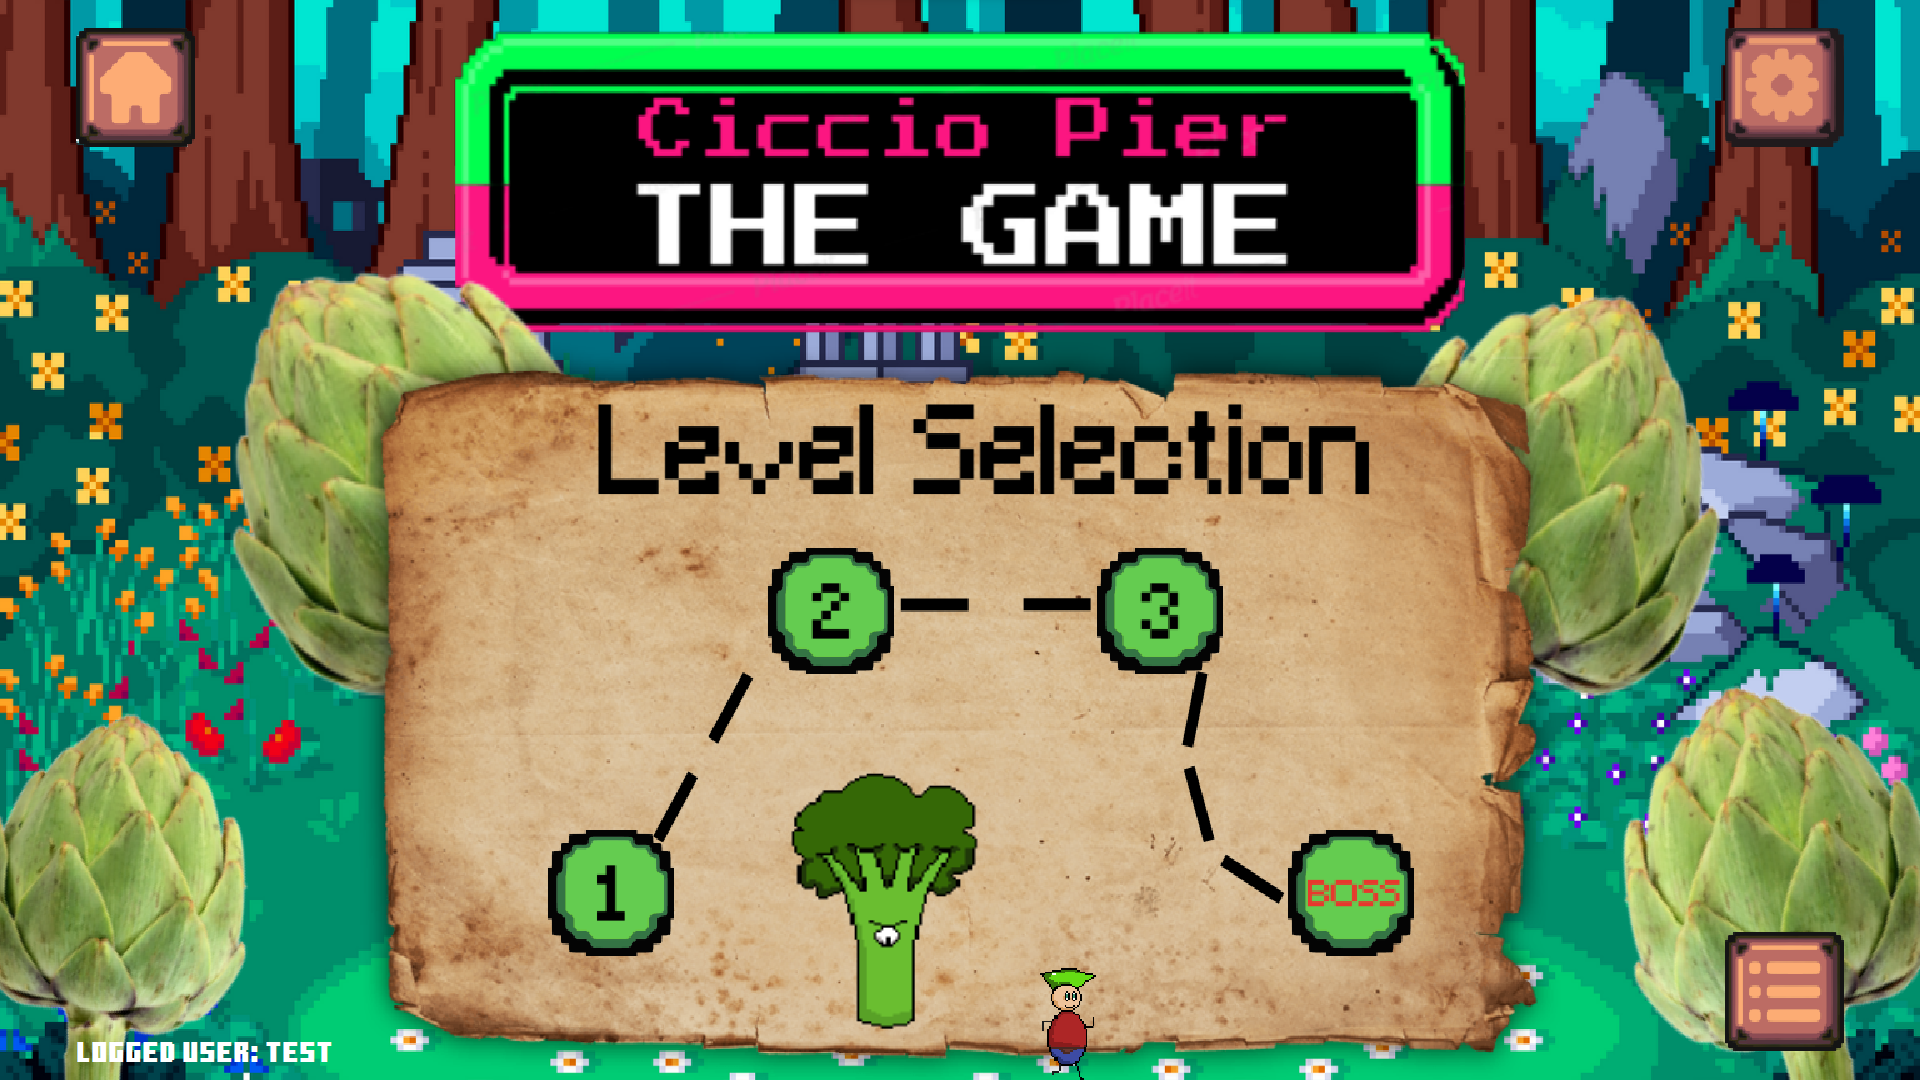
\includegraphics[scale=0.2] {img/game-selection.png}
        \caption{Schermata di selezione del livello.}
        \label{img:game-selection}
    \end{figure}

    \begin{figure}[H]
        \centering{}
        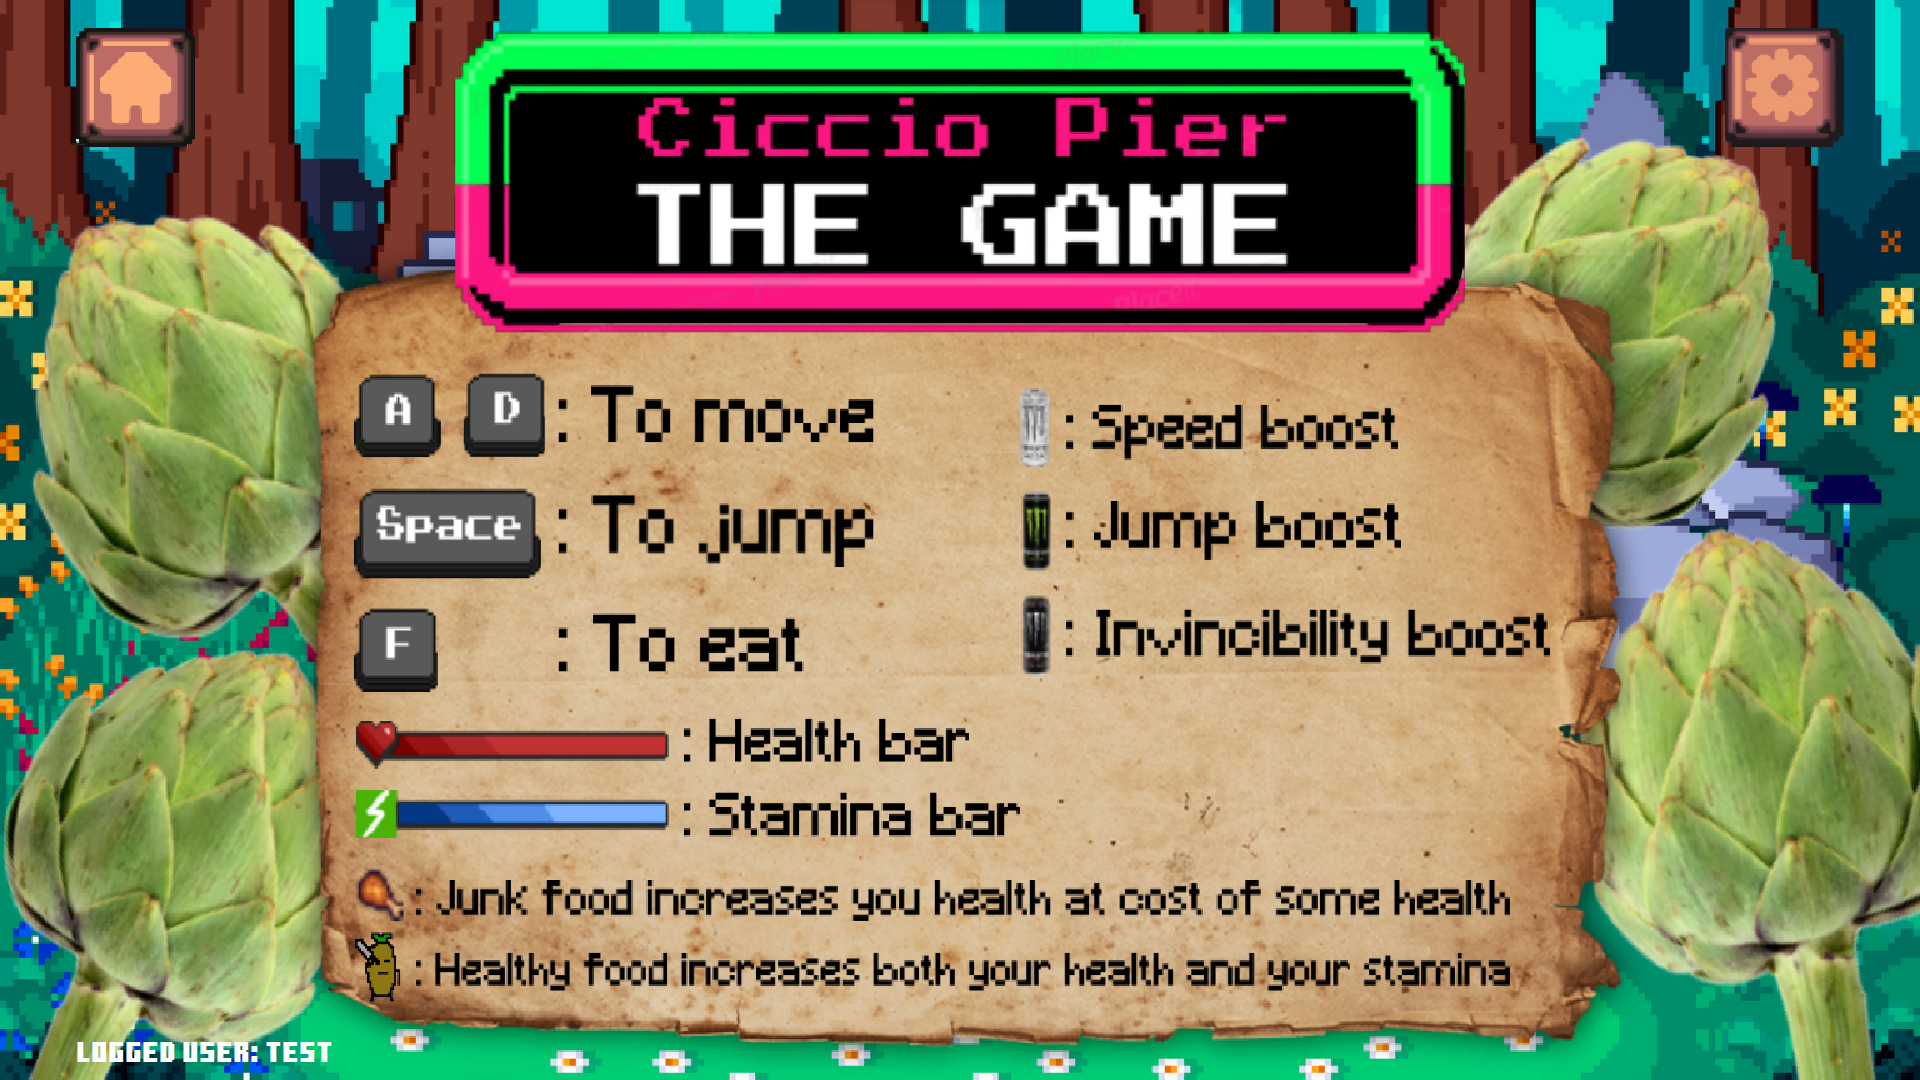
\includegraphics[scale=0.2] {img/game-tutorial.png}
        \caption{Schermata di tutorial del gioco.}
        \label{img:game-tutorial}
    \end{figure}

    Per mettere in pausa mentre si sta giocando un livello basta premere ESC.

    \bibliographystyle{alpha}
    \bibliography{13-template}

\end{document}